
\label{sec:qualitative_f}

%\arsh{Table \ref{tab:ablation} shows impact of some of the contextual signals on model performance for the Cable validation dataset. We observe that previous intents are the most important contextual signals for model performance, where we see a drop of 16.51\% in IC and 12.72\% on the SL task while the rest of the signals previous dialog Acts and previous slots have minimal impact. Further experiments showed that the choice of contextual signals is dependent upon the dataset. Our model facilitates switching of these contextual signals.}

Table \ref{tab:ablation} shows impact of some of the contextual signals on model performance for the Booking validation dataset.
As expected, contextual signals improve IC and SL performance (Configs - II-V). We observe that adding intent history ($\text{I}_{\text{hist}}$) leads to highest gains in IC accuracy (Config - IV).
%We observe that intent history is the most important contextual signal as it leads to higher gains in IC as compared to other signals (Config - IV). Other contextual signals like utterance history, dialog acts also improve IC and SL performance (Configs - II, III). 
At the same time, we see that slot history ($\text{SL}_{\text{hist}}$)  has minimal impact on SL performance for this dataset.  Exhaustive experiments showed that the choice of contextual signals is dependent upon the dataset. Our model facilitates switching these contextual signals on or off easily.

% \begin{table}[ht]
% \small
% \begin{tabular}{lcc}
% \hline
% \textbf{Configuration}      & $F1_{IC}(\%)$ & $F1_{SL}(\%)$ \\
% \hline
% \pretty{Casa-Nlu}                    & 73.70              & 66.68               \\
% - Previous Intents           & {\bf 57.19}               & {\bf 53.96}               \\
% - Previous Dialog Acts       & 73.17               & 66.72               \\
% %- Previous Utterances        & 74.81               & 67.79               \\
% - Previous Slots        & 74.53               & 66.02               \\
% \hline
% \end{tabular}
% \caption {Ablation Study on Cable validation set using \pretty{Casa-Nlu} model}
% \label{tab:ablation}
% \end{table}

\begin{table}[ht]
\small
\setlength\tabcolsep{4pt} 
\begin{tabular}{lcccccc}
\hline
\textbf{Config} & 
$\text{I}_{\text{hist}}$ & 
$\text{SL}_{\text{hist}}$ &
$\text{Utt}_{\text{hist}}$ &
$\text{DA}_{\text{hist}}$ &
\text{$\text{IC}$} & \text{$\text{SL}$} \\
%\text{$\text{F1}_{IC}$} & \text{$\text{F1}_{SL}$} \\
\hline
I   &x  &x  &x  &x  &89.44  &97.62 \\
II   &x  &x  &\checkmark  &x  &92.52  &98.09 \\
III   &x  &\checkmark  &\checkmark  &\checkmark  &92.35  &98.33 \\
IV   &\checkmark  &\checkmark  &\checkmark  &x  &95.27  &98.34 \\
%IV   &\checkmark  &x  &\checkmark  &\checkmark  &98.25  &98.42 \\
V   &\checkmark  &\checkmark  &\checkmark  &\checkmark  &96.53  &98.25 \\

\hline
\end{tabular}
\caption {Impact of contextual signals on IC accuracy and SL F1 scores (\%) on Booking validation set for \pretty{Casa-nlu}}
\label{tab:ablation}
\end{table}

\textbf{Qualitative Analysis:} 
Using example conversation in Figure~\ref{tease}, we highlight the relevance of contextual information in making intent predictions
%\glalwani{\sout{and slot}} predictions\glalwani{\sout{. We visualize}
by visualizing attention weights  $\mathbf{P}(\mathbf{T})$ (Equation \ref{eq:attn}) for different contextual signals as shown in Figure \ref{attn_1}.\footnote{For each context signal, attention weights are averaged across all its feature dimensions in $\textbf{P}(\textbf{T})$}
%\glalwani{\footnote{Attention weights are averaged across all the dimensions for corresponding context signal}}
At user turn \#2, the \emph{intent} is switched to \emph{UpgradeService} which the model successfully interprets by paying less attention to previous intents. % At the same time, model learns to attend comparatively more to the current utterance than previous utterances. 
%\textit{``increase my data plan please"} than previous utterances including \textit{``uh help"}. 
% and almost equal attention to both previous, \textit{``uh help"} and current utterance, \textit{``increase my data plan please"} \glalwani{\sout{as shown in Figure \ref{attn_1} (left)}}.
At turn \#3, however, contextual information is critical as user responds to elicitation by agent 
% \glalwani{\sout{. Figure \ref{attn_1} (right) shows} and hence model} 
and hence model emphasizes on %\glalwani{\sout{previous} last} 
last utterance and intent rather than the current or other previous turns.
%\glalwani{or other previous turns.}

% Since contextual information provides turn-level information, in this section, we show the attention map respect to each signal to see if they attend to the correct dialog turns. We focus on two signals: previous utterances and previous intents. 
%  Source2token layer aggregates all the information and helps the model to attend important parts, we thus take its output as learned attention masks. As one of evaluation set instances of Cable dataset, we take the conversation in figure~\ref{} as an example and show the results in figure~\ref{attn_1}. 
%  There is an intent switching(foot note) at turn 2. Previous intent signal attends a lot on current utterance (UpgradeService intent), which is very relevant to current intent, while previous utterance signal gets weight divided between current turn and previous turn, since both of the utterances (\textit{"increase my data plan please"} and \textit{"uh help"}) are important to understand what the user wants to convey. At turn 3, user follows up with additional information about the original request as elicited by agent. Both of these signals learn to give more attention to previous utterance and intent rather than the current turn.

\begin{figure}[h]
\centering
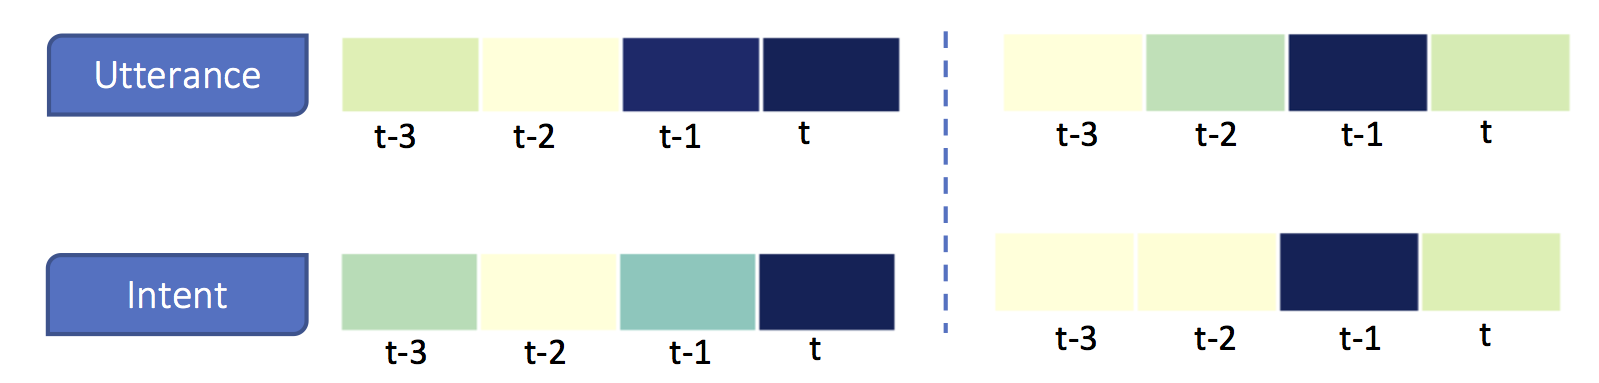
\includegraphics[width=0.5\textwidth, height=50pt]{figures/context_viz_high_res_cropped.png}
\caption{\label{attn_1} \small \textbf{Visualization of attention weights} given to two different context signals - previous utterances (top) and previous intents (bottom) for turns t=2 (left) and t=3 (right) from Figure~\ref{tease};
%here context window=3
darker colors reflect higher attention weights.}
\end{figure}
\vspace{-10pt}
% \textbf{Ablation study:} Table \ref{tab:ablation} shows impact of some of the contextual signals on model performance for the Cable validation dataset. We observe that previous intents are the most important contextual signals for model performance, where we see a drop of 16.51\% in \pretty{Ic} and 12.72\% on the \pretty{Sl} task while the rest of the signals previous dialog Acts and previous slots have minimal impact. 
%ALl this is a weird result, you would want to show that previous slots and DA have an impact otherwise, I would naturally ask, what if I had a model that only models previous intent alone?? Have you run experiments with just that signal on. This weakens the argument for using these signals. DO you have studies that have just one signal at a time?

%%ALL this next paragraph needs to be rewritten and supported with numbers 
%Despite having many single token utterances in this data set, \pretty{Casa-Nlu} is able to mitigate this problem due to the multi-dim attention as it learns which signals to emphasize for each turn.
%Interestingly, previous utterances have adverse impact on model performance for cable data as we notice that in our dataset, many of the followup utterances are single tokens and are adding confusion to the model. 
% Due to the multi-dim attention in our model, model is able to mitigate this noisy signal to a large extent.

% \begin{table}[h]
% \begin{center}
% \setlength\tabcolsep{3.5pt} 
% \begin{tabular}{@{}lcccc@{}}
% \hline
% \bf Model & \multicolumn{2}{@{}c@{}}{\bf Booking} & \multicolumn{2}{@{}c@{}}{\bf Cable} \\
% \hline
%  & F1_{First} & F1_{F/U} & F1_{First} & F1_{F/U} \\
% \hline
%   non-contextual & 95.67 & 89.51 & 40.35 & 48.33 \\
%   gru-contextual & 98.93 & 94.24 & 46.6  & 72.22 \\
%   \hline
%   \pretty{Casa-Nlu} & \textbf{99.70}  & \textbf{94.45}  & \textbf{47.44}  & \textbf{81.25} \\
% \hline
% \end{tabular}
% \end{center}
% \vspace{-7pt}
% \caption {Breakdown of \pretty{Ic} F1 scores (\%) for all the three models on two datasets into First turn and Follow-up (F/U) turns}
% \label{tab:saca_divided_results}
% \vspace{-10pt}
% \end{table}

% \begin{table}[ht]
% \small
% \begin{tabular}{lcc}
% \hline
% \textbf{Configuration}      & $F1_{IC}(\%)$ & $F1_{SL}(\%)$ \\
% \hline
% \pretty{Casa-Nlu}                    & 73.70              & 66.68               \\
% - Previous Intents           & {\bf 57.19}               & {\bf 53.96}               \\
% - Previous Dialog Acts       & 73.17               & 66.72               \\
% %- Previous Utterances        & 74.81               & 67.79               \\
% - Previous Slots        & 74.53               & 66.02               \\
% \hline
% \end{tabular}
% \caption {Ablation Study on Cable validation set using \pretty{Casa-Nlu} model}
% \label{tab:ablation}
% \end{table}
%\vspace{-10pt}




 

